%% V1.0
%% by Christopher Leith, udacl@cielsystems.com
%% This is a template for Udacity projects using IEEEtran.cls

\documentclass[10pt,journal,compsoc]{IEEEtran}

\usepackage[pdftex]{graphicx}    
\usepackage{cite}
\hyphenation{op-tical net-works semi-conduc-tor}

\begin{document}

\title{WhereAmI - Robotic Localization}

\author{Christopher Leith}

\markboth{WhereAmI, Localization, Udacity}%
{}
\IEEEtitleabstractindextext{%

\begin{abstract}
In this project we create a simulated robot and demonstrate Adaptive Monte Carlo Localization (AMCL) within the ROS framework to permit navigation within a small simulated "Gazebo" world. A differential drive robot is designed to operate within the Gazebo simulation and uses the ROS navigation stack and the AMCL package for localization within the supplied map. The RViz visualization tool is used to observe the the robot and the relevant paths, maps and point clouds as it moves to a predefined goal. The tuning of configuration parameters of the simulation, navigation stack and AMCL package neccesary for success are discussed.
\end{abstract}

% Note that keywords are not normally used for peerreview papers.
\begin{IEEEkeywords}
Mobile Robot, Localization, Monte Carlo Localiztion, ROS.
\end{IEEEkeywords}}


\maketitle
\IEEEdisplaynontitleabstractindextext
\IEEEpeerreviewmaketitle
\section{Introduction}
\IEEEPARstart{M}{obile} robots must be able to determine their location within their region of operation, a process known as localization, and navigate to other locations reliably in order to perform their tasks succesfully. \hfill \vspace{\baselineskip}

The process of robotic localization requires a known, predefined 'ground truth' map within which the robot, using sensors of various kinds, must establish the exact coordinates, in our case 2D coordinates, of its current location as it moves about the map. The are 3 primary categories of localization, in order of increasing complexity: 'local', 'global' and what is termed 'kidnapped robot' localization.  \hfill \vspace{\baselineskip}

In 'local localization' a robot's position is initially known and the robot must only keep track of its changing location as it moves. In 'global localization' the robot does not initially know its location within the map and must, over time, resolve its location using information from its sensors and the ground truth map. In 'kidnapped robot' localization the robot must always assume that its believed location could be grossly in error and must constantly recalculate its location anew. \hfill \vspace{\baselineskip}

In this project only the simple 'local localization' is demonstrated. That is, the initial location is known accurately and the robot must keep track of its location as it moves.

\label{sec:introduction}
\section{Background / Formulation}
Because localization is so important for mobile robotics it is a highly researched field and has many well developed techniques and technologies. Most people are familiar with the Global Positioning System (GPS) which permits an electronic device to directly infer its latitude, longitude and altitude based on signals received from GPS satellites. Other techniques such as Kalman filtering and Monte Carlo Localization (aka 'Particle Filter') are techniques that can take input from a variety of sensors and over time compute estimates of the current location. Such sensors include radar, laser scanners, cameras, odometry sensors, Inertial Measurement Units (IMU), sonar, compass sensors and more. In many cases multiple sensor inputs are used simulataneously with theses techniques in a process known as Sensor Fusion. Selecting techniques and sensors is part of the complicated design process of a robot and of course depends on the intended application, the intended environment, eg indoor or outdoor, and the typical engineering constraints of cost, size, power, sensor noise, computational power, and required reliability and performance goals.  \hfill \vspace{\baselineskip}

For this simulation project we are, fortunately, given absolute constraints on all of these design considerations. Specifically the robot is to be a wheeled, differential drive robot operating in a small, flat, 2D environment with only noiseless wheel odometry sensors and a laser scanner and we will discuss only the Kalman filter Monte Carlo Localization techniques and only implement to Monte Carlo technique. Furthermore the application is to occur in a ROS Gazebo simulated environment with a predfined, known 'ground truth' map and a very simple objective of navigating to a predefined goal location.  \hfill \vspace{\baselineskip}

This simple robot objective is, of course, merely a context for the wider objective of learning about some techiques and technologies of mobile robotic design. Specifically we are gaining knowledge of the using ROS robotics framework for robotic system design and the the ROS Gazebo simulation environment for design R\&D and test and using the ROS Adaptive Monte Carlo Localization (AMCL) package with odometry and laser scanner sensors to learn about important parameter tuning considerations. 

\subsection{Kalman Filter}
Subsection

\subsection{Adaptive Monte Carlo Localization}
Subsection

\section{Results}
Results

\subsection{Udacity-Bot}
The initial spread of Monte Carlo particles can be seen. (Fig ~\ref{fig:UdaBot Initial Particles})
The converged Monte Carlo particles at the goal can be seen. (Fig ~\ref{fig:UdaBot Goal Particles})

\begin{figure}[h]
      \centering
      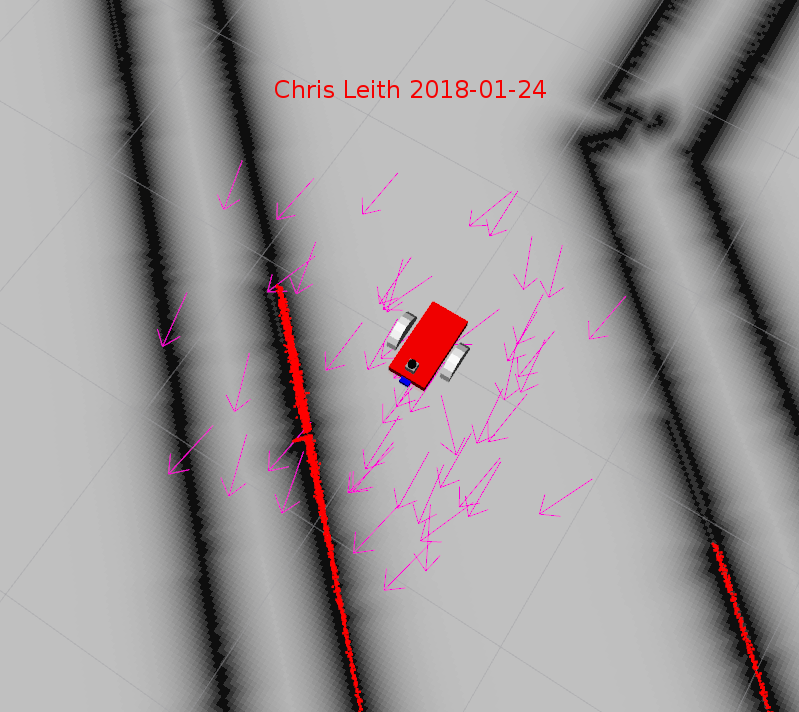
\includegraphics[width=\linewidth]{../Assets/writeupImages/udaBot_rvizInit.png}
      \caption{UdaBot Initial Particles }
      \label{fig:UdaBot Initial Particles}
\end{figure}

\begin{figure}[h]
      \centering
      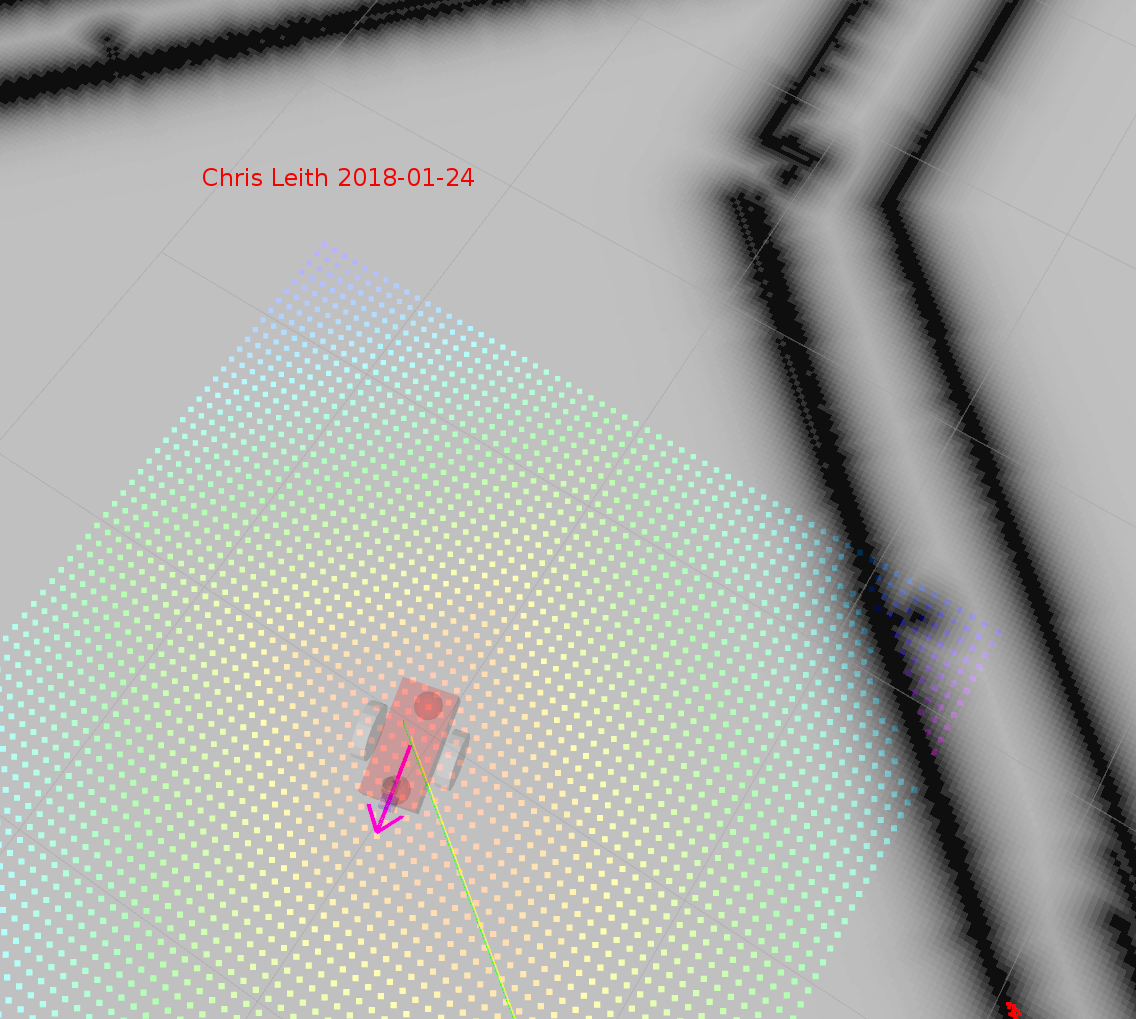
\includegraphics[width=\linewidth]{../Assets/writeupImages/udaBot_rvizGoal.png}
      \caption{UdaBot Goal Particles }
      \label{fig:UdaBot Goal Particles}
\end{figure}

\subsection{Ciel-Bot}
The initial spread of Monte Carlo particles can be seen. (Fig ~\ref{fig:CielBot Initial Particles})
The converged Monte Carlo particles at the goal can be seen. (Fig ~\ref{fig:CielBot Goal Particles})

\begin{figure}[h]
      \centering
      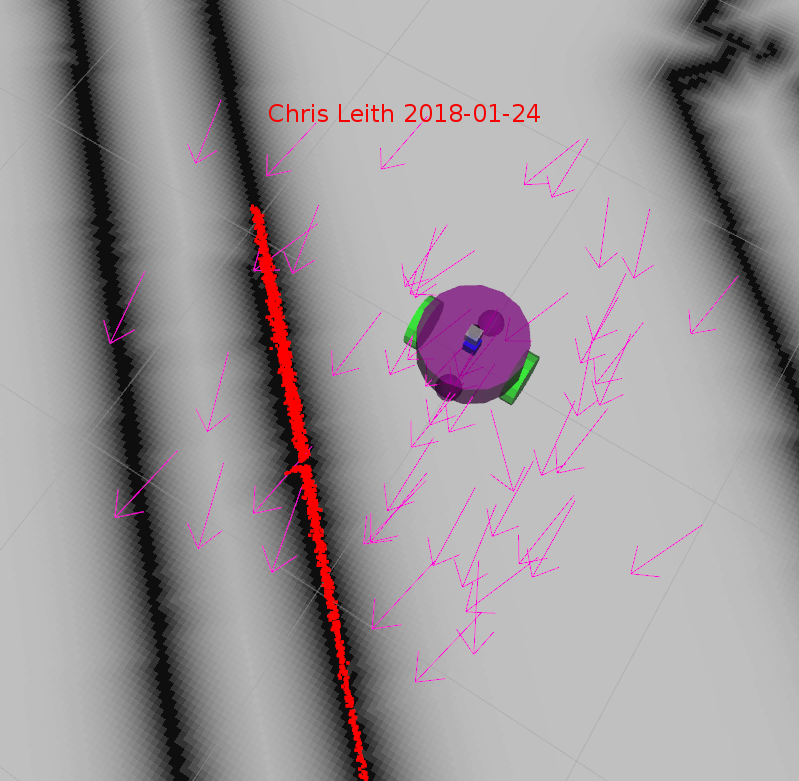
\includegraphics[width=\linewidth]{../Assets/writeupImages/cielBot_rvizInit.png}
      \caption{cielBot Initial Particles }
      \label{fig:cielBot Initial Particles}
\end{figure}

\begin{figure}[h]
      \centering
      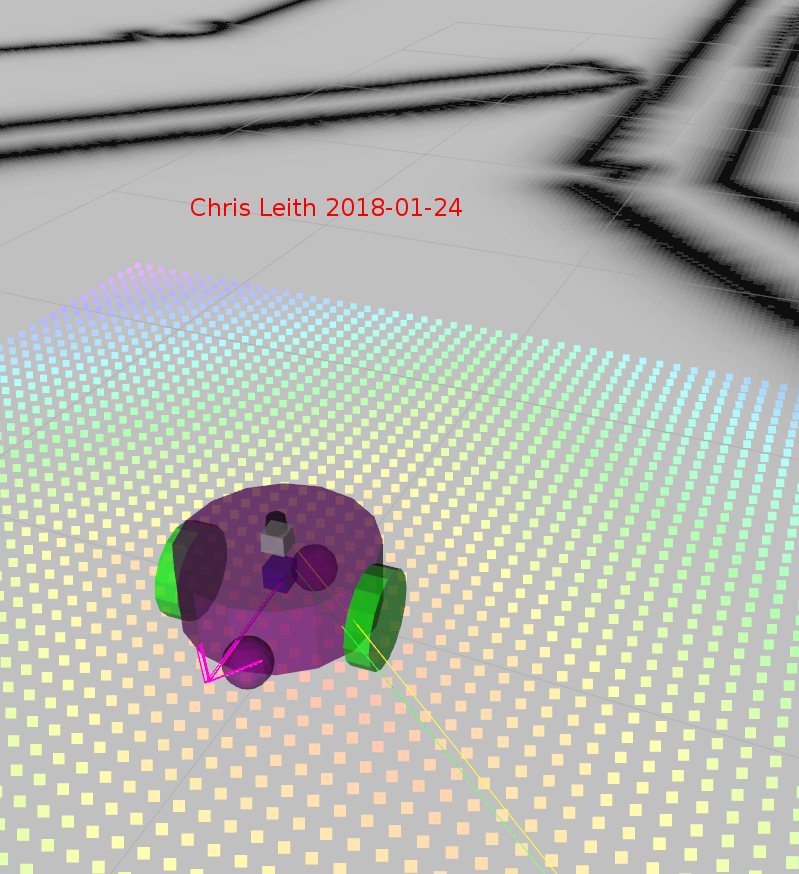
\includegraphics[width=\linewidth]{../Assets/writeupImages/cielBot_rvizGoal.png}
      \caption{cielBot Goal Particles }
      \label{fig:cielBot Goal Particles}
\end{figure}


\section{Model Configuration}
Model Configuration

\subsection{Udacity-Bot}
Subsection

\subsection{Ciel-Bot}
Subsection


\section{Discussion}
Discussion

\section{Conclusion / Future work}
Conclusion

\end{document}